\subsection{黄河流域概况}

黄河流域($95^{\circ}52'37” \sim 119^{\circ}3'56”E$,$32^{\circ}9'38” \sim 41^{\circ}51'37”N$)跨越三个气候带,气候和生态系统类型复杂,干流流程$5.4 \times 10^3~km$、流域面积$76.6 \times 10^4~km^2$,约为中国国土面积的$8.3\%$,是中国第二大流域。
黄河流域大部分位于我国干旱半干旱地区,年平均温度约为$6.4 ^{\circ}C$,潜在蒸发量超过$800~mm$,年均降水量不足$500~mm$且季节差异明显,中游以上流域夏季降水量可占全年降水量的$85\%$\cite{maxuening2012,wang2007}。
黄河流域地形变化较大,流域海拔变化超过$6200~m$,水面海拔高度差达$4480~m$。
流域内多样复杂的地形让黄河流域上、中、下游地理条件相差极大,且具有无以伦比的独特性:上游是世界上最年轻/快速隆升的青藏高原;中游是唯一正在堆积/强烈剥蚀的黄土高原;下游供给着人口密集/水资源需求极大的华北平原。
上游与源区最大的生态系统功能是水源涵养,黄河$534.79$亿立方米的多年平均地表水资源量中,有$60\%$以上来水来自兰州以上的源区\cite{huchunhong2018}。
中游黄土易垦区在人类活动和气候变化的双重影响下,因植被破坏和水土流失产生的泥沙让黄河曾以泥沙输运量最高的河流而闻名于世\cite{best2019}。
而在花园口站以下的黄河下游区域,因泥沙沉积抬高高程而形成了地上悬河,流域面积仅为$3 \times 10^4~km^2$,产流量低,且主河道在历史时期因频繁的洪泛决溢而在华北平原上频繁摆动,自西向东形成不计其数的辫状古河道。


\begin{figure}[!ht] % use float package if you want it here
    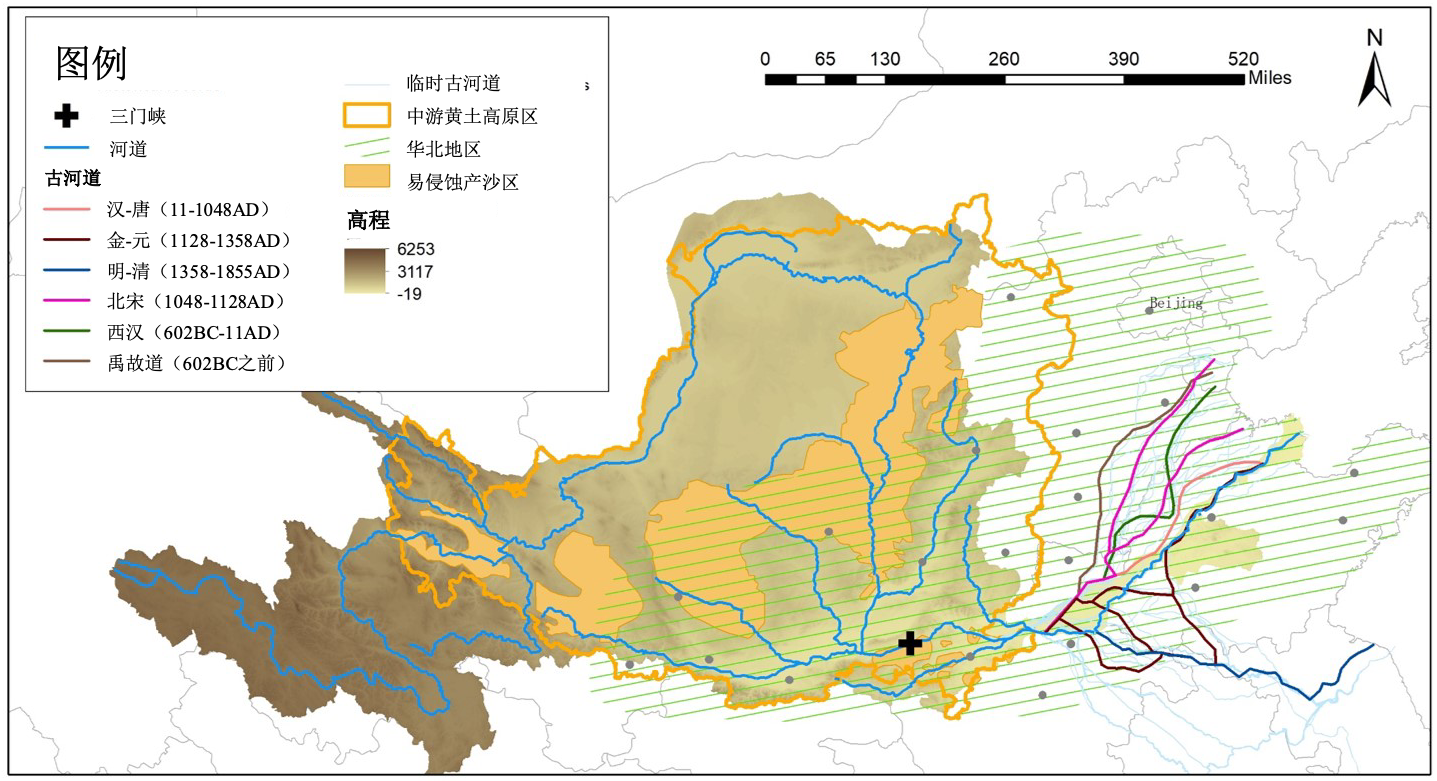
\includegraphics[width=\textwidth]{img/ch1/ch1_study_area.png}
    \caption{黄河流域研究区示意图}\label{ch1:fig:study_area}
\end{figure}

黄河流域历经了三千多年的开发和近现代的高强度经济活动影响,导致人类活动与资源环境之间的关系不断发生变化\cite{fu2021a}。
随着人口的增长,中游黄土高原地区的耕种面积不断扩大,甚至发展到了丘陵和陡坡地区,造成了严重的水土流失,导致黄河的泥沙输送量急剧增加\cite{wu2020a}。
这些泥沙在下游造成了地上悬河,导致洪泛决溢频繁发生,给黄河中下游的社会经济带来了灾难,例如宋朝和清朝都花费了大量的人力物力在黄河流域的救灾上。
从二十世纪中期以来,随着灌溉和水库技术的成熟和农业技术的进步,黄河下游逐渐从泛滥成灾变成了造福国家和人民的粮仓,但是同时也出现了“水少”的问题。
农业灌溉水资源的开发已接近极限,抽取的水量接近地表径流的 $8\%$,导致黄河自 $1972$ 年以来频繁断流,出现了日益严重的水资源危机。
黄河流域是中国重要的农业和工业生产基地,人口稠密,社会经济活动密集。随着工业和服务业用水需求的增加,人-水-食物-能源的关系变得更加复杂,因此有必要根据人-水系统的反馈循环,以长远和动态的眼光实现人-水关系的和谐,以实现流域的高质量、可持续发展。

\subsection{黄河流域治理简史}

历史上,黄河流域的水治理一直是人-水关系不断变化的重要驱动力。自有记录的历史以来,中央王朝就已经为治理黄河积累了大量的文献资料,并被视为关乎国家长治久安的重大任务。
在西汉中后期,随着河道淤积和河患增加,各种治河思想已经非常活跃。史料表明,在著名的“王景治河”时期,黄河下游已经普遍建有完备的堤防建设\cite{WangWeiJing2009}。
在王景治河之后,黄河流顺数世纪,直到北宋到元代重新进入了有史以来水患最严重的一段时期。频繁的河道变迁和堤防决溢迫使宋朝政府广泛征集治河水利人才,并建立岁修制度和治河责任制,但治河的总方针在“恢复东流”和“北流入海”之间的争执无法解决,因此国家大量的资金和粮食被用于河道作业和救灾\cite{WangWeiJing2009, yang2019}。
在明代,随着黄河泛滥的趋势逐渐缓解,河流治理主要是为了保护京杭大运河的漕运服务。当时采用了潘季驯的“束水攻沙”思想,初步认识到水沙关系的重要性\cite{WangWeiJing2009}。
在清朝前期,国力强盛时也有“汰沙澄源”的提议,重视水保,但未受到重视,因此政府仍然继续沿用古人思想进行治理,并将大运河与黄河分离,使漕运和治河并重。然而,随着清王朝中后期国力的逐渐衰弱,政府不再能承受这种黄河治理的压力,最终导致了又一次决堤,使黄河离开了七百年来南流夺淮的河道\cite{WangWeiJing2009}。


进入现代中国,科学认识的加深带来了“治黄先治沙”的治理方针,随后的一系列工程措施,如水库、淤地坝、渠道等,使得黄河的年平均泥沙输运量在六十年内降至原来的十分之一,缓解了困扰数千年的高输沙量和高淤积量问题\cite{wang2016a}。
面对水资源短缺等新的挑战,黄河流域采取了一系列有力的治理措施,包括工程措施(如水库联合调控、南水北调)和制度法规(如“水资源配额制度”、“最严格水资源管理”、《黄河流域保护法》等)\cite{shuilibuhuangheshuiliweiyuanhui2010}。
水资源配额制度对黄河流域的影响最为深远,从1980年首次提出到现在,它一直是指导和限制各地区用水的关键,比如联合调度、最严格水资源管理等都是在该方案的基础上执行的,尽管有多个省份认为该方案与实际情况越来越不符\cite{wang2019b,wang2019e}。
2019年9月的黄河流域生态保护和高质量发展座谈会上,黄河流域生态保护和高质量发展被正式定为国家重要战略,强调需要“重塑人-水关系”和“坚守生态保护红线”。同年,黄河水资源分配制度的调整被列为当务之急;2022年,《黄河保护法》正式通过\cite{lu2019,dongzhanfeng2020}。
这些新举措表明,“治好黄河”的方向和决心一直没有改变。了解黄河流域人-水关系的变化和机制,分析流域管理实践对人-水关系的影响机制,将有助于在全球变化不断加剧的环境中,为黄河高质量和可持续发展提供科学依据。
